\section{Design}

The astable oscillator configuration of the~555 timer can be constructed using
the configuration shown in Figure~\ref{f:astable}.
%
\begin{figure}[H]
\centering
	\includegraphics[width=.6\textwidth]{img/shot/555schem.pdf}
	\parbox{.6\textwidth}{
	\caption[Astable Oscillator Schematic]{Schematic for a 555 timer-based
	astable oscillator, as provided by the lab instructions.}
	\label{f:astable}}
\end{figure}
%
This schematic, included in the lab instructions, utilizes the
elements~$R_A$,~$R_B$, and~$C$ to generate a square wave across the output
terminal of the chip.  The frequency and duty cycle of said output are set by
carefully choosing the external elements shown in Figure~\ref{f:astable},
according to~\eqref{eq:f} and~\eqref{eq:duty}.
%
\begin{align}
	f &= \frac{1}{ \left( R_A + 2 R_B \right) C \ln{2} } \label{eq:f}\\
	\text{Duty Cycle} &= \frac{R_A + R_B}{R_A + 2 R_B} \times 100\% \label{eq:duty}
\end{align}
%
Students were provided a target frequency of~\SI{8}{\kilo\hertz} and a target
duty cycle of~\SI{90}{\percent}, and thus calculated element values appropriately.

To aid in the calculation process, the 555 timer datasheet provided a graph of
required capacitor versus frequency for a variety of resistor combinations.
This plot has been reproduced in Figure~\ref{f:cap_graph}.
%
\begin{figure}[H]
\centering
	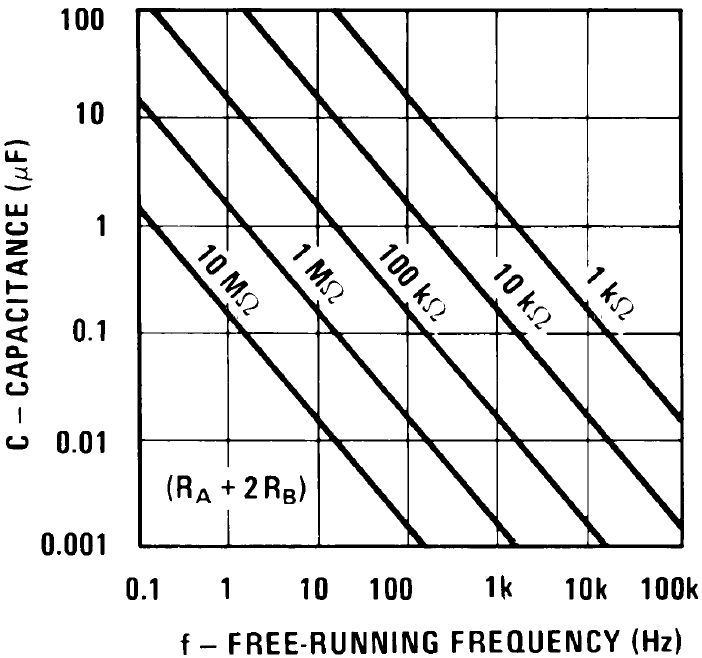
\includegraphics[width=.6\textwidth]{img/shot/555_graph.png}
	\parbox{.6\textwidth}{
	\caption[Datasheet Aide Graph]{Graph included in the~555 timer's datasheet
	to aid in the selection of appropriate element values.}
	\label{f:cap_graph}}
\end{figure}
%
Because~\SI{10}{\nano\farad} capacitors are very easily-obtainable, this was
the value of~$C$ chosen.  When combined with the~\SI{8}{\kilo\hertz} target
frequency, the required value of~$R_A + 2 R_B$ was~\SI{20}{\kilo\ohm}.  This
value was then used in~\eqref{eq:duty}:
%
\begin{align*}
	\left( R_A + 2 R_B \right) \cdot \frac{\text{Duty Cycle}}{100} &= R_A + R_B \\
	\SI{20}{\kilo\ohm} \cdot 0.90 &= R_A + R_B \\
	\SI{18}{\kilo\ohm} &= R_A + R_B
\end{align*}

The resulting system of equations can be solved, producing resistances
for~$R_A$ and~$R_B$:
%
\begin{align*}
	R_A + R_B &= \SI{18}{\kilo\ohm} \\
	R_A + 2R_B &= \SI{20}{\kilo\ohm} \\
	&\therefore \\
	R_B &= \SI{2}{\kilo\ohm} \\
	R_A &= \SI{16}{\kilo\ohm} \\
\end{align*}

Unfortunately for the student, the calculated resistances were invalidated
after reading the lab instructions, as the course instructor also provided
appropriate values for these elements.  Students obtained each of~$R_A$,~$R_B$,
and~$C$ as a~\SI{14.4}{\kilo\ohm} resistor, a~\SI{1.8}{\kilo\ohm} resistor, and
a~\SI{10}{\nano\farad} capacitor; the measured values for each are shown in
Table~\ref{t:elements}.
%
\begin{table}[H]
	\centering
	\parbox{.5\textwidth}{
	\caption[Element Values]{Required, nominal, and measured values for the
	external elements used to create the 555-based clock.  Note that these are
	the element values provided by the lab instructors.}
	\label{t:elements}}\\
	\section{Elements}

After consulting the datasheet for the DAC0808 integrated circuit, it was
determined that three~\SI{5}{\kilo\ohm} resistors were required for the proper
operation of the chip.  The measured values are shown in
Table~\ref{t:elements}, along with the elements used in the construction of the
ADC in step 2 (which utilized the ADC0804 IC).
%
\begin{table}[H]
\centering
	\section{Elements}

After consulting the datasheet for the DAC0808 integrated circuit, it was
determined that three~\SI{5}{\kilo\ohm} resistors were required for the proper
operation of the chip.  The measured values are shown in
Table~\ref{t:elements}, along with the elements used in the construction of the
ADC in step 2 (which utilized the ADC0804 IC).
%
\begin{table}[H]
\centering
	\section{Elements}

After consulting the datasheet for the DAC0808 integrated circuit, it was
determined that three~\SI{5}{\kilo\ohm} resistors were required for the proper
operation of the chip.  The measured values are shown in
Table~\ref{t:elements}, along with the elements used in the construction of the
ADC in step 2 (which utilized the ADC0804 IC).
%
\begin{table}[H]
\centering
	\input{tbl/elements.tex}
	\parbox{.8\textwidth}{
	\caption[List of used elements]{Required, nominal, and measured element
	values used in the ADC and DAC circuits.}
	\label{t:elements}}
\end{table}
%
With errors for the DAC resistors all falling under~\SI{1}{\percent}, the
elements are all appropriately accurate for this application.

	\parbox{.8\textwidth}{
	\caption[List of used elements]{Required, nominal, and measured element
	values used in the ADC and DAC circuits.}
	\label{t:elements}}
\end{table}
%
With errors for the DAC resistors all falling under~\SI{1}{\percent}, the
elements are all appropriately accurate for this application.

	\parbox{.8\textwidth}{
	\caption[List of used elements]{Required, nominal, and measured element
	values used in the ADC and DAC circuits.}
	\label{t:elements}}
\end{table}
%
With errors for the DAC resistors all falling under~\SI{1}{\percent}, the
elements are all appropriately accurate for this application.

\end{table}
